\section{Modelos de grano grueso}\label{sec:Ch1CG}

\subsection{Descripciones efectivas}

\acnote{Sección iterada: reescritura, requiere revisión.}

 \acnote{Sección iterada: notas}

En nuestro día a día no podemos procesar toda la información de todos los sistemas con los que interactuamos: no nos preocupa la energía cinética individual de cada una de las moléculas de agua presente en cada una de las gotas que caen sobre nosotros, sino qué tan caliente o frío parece el chorro que sale de la llave. Una descripción de \textit{grano grueso} es aquella que no toma en cuenta todos los detalles de un sistema o fenómeno. Estas particularidades microscópicas suelen omitirse ya sea por la incapacidad del observador de procesar toda la información asociada a estas, o de no tener acceso a todos los grados de libertad de dicho sistema.

El conjunto de variables termodinámicas de un sistema en equilibrio térmico puede verse como una descripción efectiva de una realidad microscópica subyacente. En este sentido, de la mecánica estadística pueden obtenerse estas variables termodinámicas como promedios de propiedades microscópicas. A las colisiones de un número estadísticamente significativo de partículas contra las paredes de un objeto se les puede promediar y reducir a una única variable: presión. De manera similar, la temperatura de un gas ideal se relaciona con la energía cinética de las partículas de este explícitamente a través de un promedio utilizando la distribución de Boltzmann. En efecto, 
\begin{equation}
    T=\frac{1}{k_\text{B}}\frac{2}{3}\expval{E_{\text{cin}}}.
\end{equation}
\begin{figure}[ht]
    \centering
    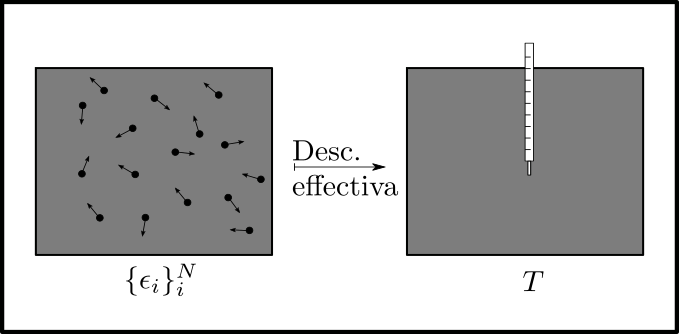
\includegraphics[width=0.6\linewidth]{chapter1/figures/CGT.png}
    \caption{Reducir las energías cinéticas individuales de $N$ partículas a un temperatura es un modelo de grano grueso}
    \label{fig:KtoT}
\end{figure}

En mecánica estadística se utiliza la estadística para pasar de una descripción fina a una gruesa, en la que cantidades arbitrariamente grandes de variables son sustituidas por distribuciones de probabilidad.

Los modelos de grano grueso son útiles porque permiten hacer predicciones sin tener que lidiar con cantidades de información que pueden ser no manejables, o simplemente no accesibles. Por esta razón, los modelos de grano grueso son comunes en física-química \cite{PhysChemI,PhysChemII,PhysChemIII} \acnote{revisar bien estos artículos}.


\subsection{Grano grueso en mecánica cuántica}

\acnote{Sección iterada, notas}

En el contexto de la mecánica cuántica, un modelo de grano grueso puede obtenerse trazando sobre un subsistema del sistema de interés. Es importante notar que el subsistema ignorado no es necesariamente una parte que puede ser separada del sistema, como en el caso de dos partículas, sino que puede representar otros grados de libertad del sistema que se deciden ignorar, por ejemplo, al describir un ión atrapado en una trampa magnetoóptica, una opción es ignorar los grados de libertad espaciales y quedarse solo con el espín total del ión \cite{Fox}. Ahora, la separación sistema-entorno no es siempre posible \cite{Macro-To-Micro}, por lo que nos limitamos a los casos en los que los grados de libertad ignorados pueden trazarse a través de la operación de traza parcial, como se discutió en la sección \ref{sec:Ch1PartialTrace}.

Un ejemplo sencillo de un modelo de grano grueso es el de un sistema de dos partículas, del cual únicamente nos importa una. En dicho caso, el modelo puede consistir en estudiar únicamente al operador de densidad reducido correspondiente a la partícula de nuestro interés. De forma general en el contexto de este trabajo, el modelo de grano grueso consiste en reducir la dimensión del sistema estudiado. En nuestro contexto, una aplicación de grano grueso $\Lambda$ es tal que manda a un operador de densidad $\varrho\in\densityspace{n}$ a algún otro operador de densidad $\rho\in\densityspace{m}$ con $m<n$. Esto es:
\begin{align}
    \mcF:\densityspace{n}\to \densityspace{m}, n>m\nonumber
\end{align}